\subsection{$\Gamma_1 = \{1\}$, $\Gamma_2 = \{2\}$}
The initial quiver is illustrated in Figure~\ref{f:h_n=3_1-2}. 
\begin{figure}[htb]
\begin{center}
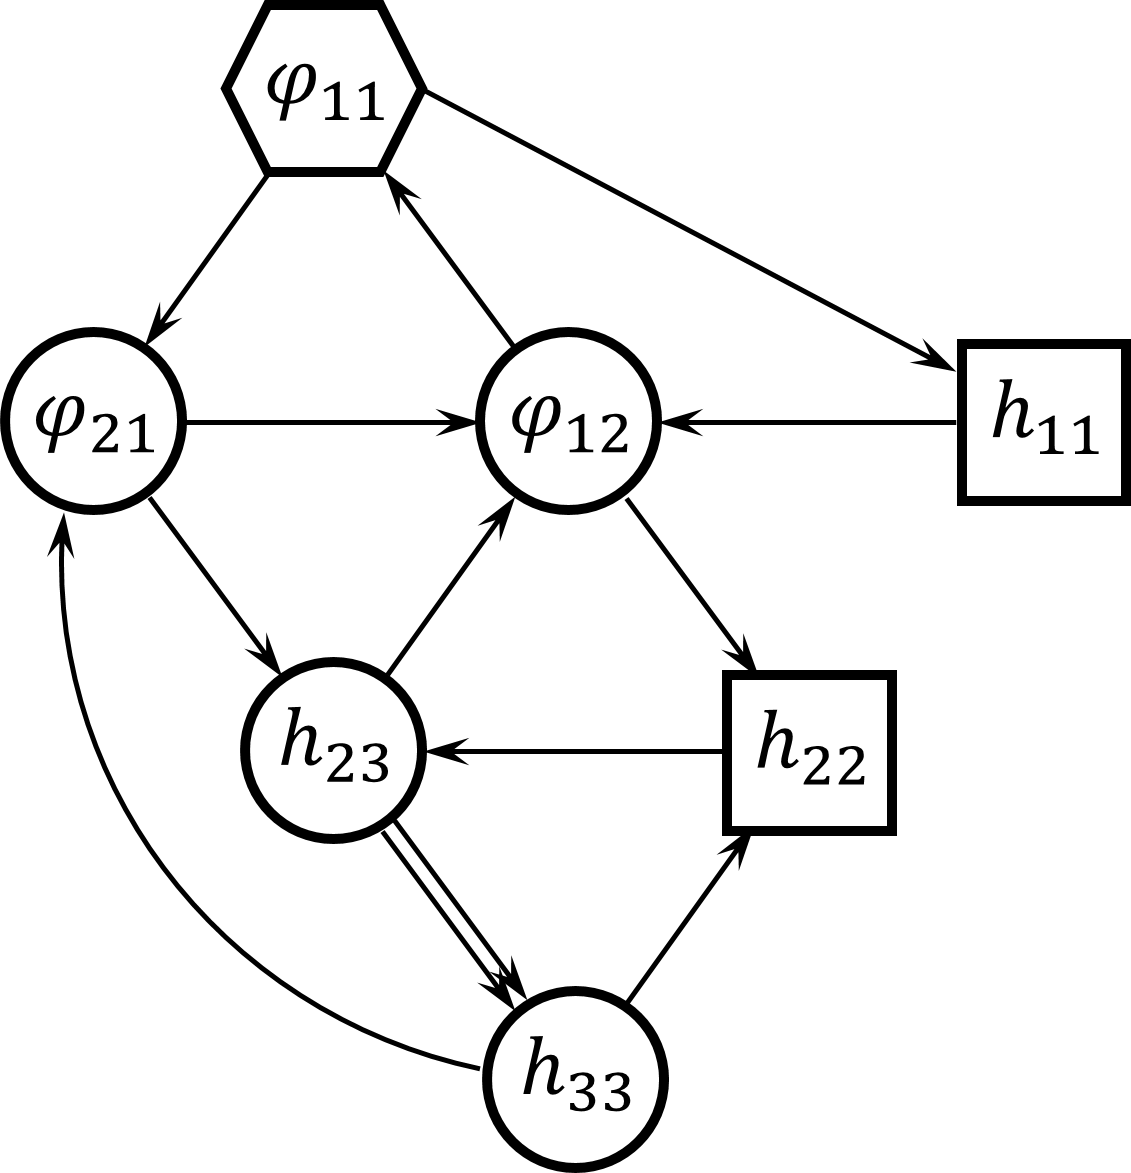
\includegraphics[scale=0.65]{h_convention/h_n=3_1-2.png}
\end{center}
\caption{The initial quiver for $\gc_h^{\dagger}(\bg,\GL_3)$ with $\Gamma_1 = \{1\}$, $\Gamma_2  = \{2\}$.}
\label{f:h_n=3_1-2}
\end{figure}

\paragraph{The initial variables.} All the variables in the initial extended cluster are as in $\gc_h^{\dagger}(\bg_{\std},\GL_3)$ except the variables $h_{23}$ and $h_{22}$; these are given by
\begin{equation}
    h_{23}(U) = -u_{23}u_{33}-u_{13}u_{32}, \ \ h_{22}(U) = u_{33} \det U^{[2,3]}_{[2,3]} + u_{32} \det U^{\{1,3\}}_{[2,3]}.
\end{equation}

\paragraph{Birational quasi-isomorphisms.} The birational quasi-isomorphism \[\mathcal{Q}:(\GL_3,\gc_h^{\dagger}(\bg_{\std}))\dashrightarrow (\GL_3,\gc_h^{\dagger}(\bg))\] is given by
\begin{equation}
    \mathcal{Q}(U) = (I-\alpha(U)e_{21})U(I+\alpha(U)e_{21}), \ \ \alpha(U):=\frac{u_{32}}{u_{33}}.
\end{equation}